%%%%%%%%%%%%%%%%%%%%%%%%%%%%%%%%%%%%%%%%%
% Short Sectioned Assignment LaTeX Template Version 1.0 (5/5/12)
% This template has been downloaded from: http://www.LaTeXTemplates.com
% Original author:  Frits Wenneker (http://www.howtotex.com)
% License: CC BY-NC-SA 3.0 (http://creativecommons.org/licenses/by-nc-sa/3.0/)
%%%%%%%%%%%%%%%%%%%%%%%%%%%%%%%%%%%%%%%%%

% \documentclass[paper=a4, fontsize=11pt]{scrartcl} % A4 paper and 11pt font size
\documentclass[11pt, a4paper]{book}
\usepackage[T1]{fontenc} % Use 8-bit encoding that has 256 glyphs
\usepackage[utf8]{inputenc}
\usepackage{fourier} % Use the Adobe Utopia font for the document - comment this line to return to the LaTeX default
\usepackage{listings} % para insertar código con formato similar al editor
\usepackage[spanish, es-tabla]{babel} % Selecciona el español para palabras introducidas automáticamente, p.ej. "septiembre" en la fecha y especifica que se use la palabra Tabla en vez de Cuadro
\usepackage{url} % ,href} %para incluir URLs e hipervínculos dentro del texto (aunque hay que instalar href)
\usepackage{graphics,graphicx, float} %para incluir imágenes y colocarlas
\usepackage[gen]{eurosym} %para incluir el símbolo del euro
\usepackage{enumerate}
\usepackage{hyperref}
\usepackage{graphicx}
\usepackage{tabularx}
\usepackage{booktabs}
\usepackage{wrapfig}

% Para las tablas
\usepackage{array}
\usepackage{colortbl}

% Para la enumeración RF-* de los requisitos funcionales
\usepackage[shortlabels]{enumitem}

\usepackage[table,xcdraw]{xcolor}
\hypersetup{
	colorlinks=true,	% false: boxed links; true: colored links
	linkcolor=black,	% color of internal links
	urlcolor=cyan		% color of external links
}
\renewcommand{\familydefault}{\sfdefault}
\usepackage{fancyhdr} % Custom headers and footers
\pagestyle{fancyplain} % Makes all pages in the document conform to the custom headers and footers
\fancyhead[L]{} % Empty left header
\fancyhead[C]{} % Empty center header
\fancyhead[R]{Pablo Cordero Romero} % My name
\fancyfoot[L]{} % Empty left footer
\fancyfoot[C]{} % Empty center footer
\fancyfoot[R]{\thepage} % Page numbering for right footer
%\renewcommand{\headrulewidth}{0pt} % Remove header underlines
\renewcommand{\footrulewidth}{0pt} % Remove footer underlines
\setlength{\headheight}{13.6pt} % Customize the height of the header

\usepackage{titlesec, blindtext, color}
\definecolor{gray75}{gray}{0.75}
\newcommand{\hsp}{\hspace{20pt}}
\titleformat{\chapter}[hang]{\Huge\bfseries}{\thechapter\hsp\textcolor{gray75}{|}\hsp}{0pt}{\Huge\bfseries}
\setcounter{secnumdepth}{4}
\usepackage[Lenny]{fncychap}

% Todo lo relacionado a citas
\usepackage{cite} %para incluir citas del archivo <nombre>.bib
% \usepackage[style=apa, backend=biber]{biblatex}
\usepackage{apacite}
\hypersetup{%
	citecolor=black
}
% \bibliographystyle{apacite} 

\begin{document}

	% Plantilla portada UGR
	\begin{titlepage}
\newlength{\centeroffset}
\setlength{\centeroffset}{-0.5\oddsidemargin}
\addtolength{\centeroffset}{0.5\evensidemargin}
\thispagestyle{empty}

\noindent\hspace*{\centeroffset}\begin{minipage}{\textwidth}

\centering

\includegraphics[width=0.9\textwidth]{logos/logo_ugr.jpg}\\[1.4cm]

\textsc{ \Large TRABAJO FIN DE GRADO\\[0.2cm]}
\textsc{ GRADO EN INGENIERIA INFORMATICA}\\[1cm]

{\Huge\bfseries Título \\}
\noindent\rule[-1ex]{\textwidth}{3pt}\\[3.5ex]
{\large\bfseries Subtítulo }
\end{minipage}

\vspace{2.5cm}
\noindent\hspace*{\centeroffset}
\begin{minipage}{\textwidth}
\centering

\textbf{Autor}\\ {Pablo Cordero Romero}\\[2.5ex]
\textbf{Director}\\ {Nuria Medina Medina}\\[2cm]

\includegraphics[width=0.3\textwidth]{logos/etsiit_logo.png}\\[0.1cm]
\textsc{Escuela Técnica Superior de Ingenierías Informática y de Telecomunicación}\\
\textsc{---}\\
Granada, Junio de 2020
\end{minipage}
\end{titlepage}


	% Plantilla prefacio UGR
	\thispagestyle{empty}

\begin{center}
{\large\bfseries Título \\ Subtítulo }\\
\end{center}
\begin{center}
	Pablo Cordero Romero\\
\end{center}

%\vspace{0.7cm}

\vspace{0.5cm}
\noindent{\textbf{Palabras clave}: \textit{software libre}
\vspace{0.7cm}

\noindent{\textbf{Resumen}\\
	

\cleardoublepage

\begin{center}
	{\large\bfseries Same, but in English}\\
\end{center}
\begin{center}
	Pablo Cordero Romero\\
\end{center}
\vspace{0.5cm}
\noindent{\textbf{Keywords}: \textit{open source}, \textit{floss}
\vspace{0.7cm}

\noindent{\textbf{Abstract}\\


\cleardoublepage

\thispagestyle{empty}

\noindent\rule[-1ex]{\textwidth}{2pt}\\[4.5ex]

D. \textbf{Tutora/e(s)}, Profesor(a) del ...

\vspace{0.5cm}

\textbf{Informo:}

\vspace{0.5cm}

Que el presente trabajo, titulado \textit{\textbf{Chief}},
ha sido realizado bajo mi supervisión por \textbf{Estudiante}, y autorizo la defensa de dicho trabajo ante el tribunal
que corresponda.

\vspace{0.5cm}

Y para que conste, expiden y firman el presente informe en Granada a Junio de 2018.

\vspace{1cm}

\textbf{El/la director(a)/es: }

\vspace{5cm}

\noindent \textbf{(nombre completo tutor/a/es)}

\chapter*{Agradecimientos}






	% Índice de contenidos
	\newpage
	\tableofcontents

	% Índice de imágenes y tablas
	\newpage
	\listoffigures

	% Si hay suficientes se incluirá dicho índice
	\listoftables 
	\newpage

	% Introducción 
	\chapter{Introducción}

Durante su labor, la \textit{Fundación Escuela de Solidaridad} ha encontrado problemas en su flujo de trabajo. Utilizando herramientas comunes, se dificultaba la gestión de la información referente a las personas a las que ayudan así como la gestión de otros tantos ámbitos de esta. Con este contexto, la fundación se planteó el buscar una alternativa que les ayudase en esta tarea.

Con esta premisa, nace el proyecto a desarrollar. Se centra en la búsqueda y desarrollo de una solución de software a los problemas que enfrenta la organización en cuanto a gestión de la información y acceso a esta. Además de esto, se busca gestionar y facilitar otras labores interesantes solicitadas por los diferentes integrantes de esta.

\section{Motivación}

El planteamiento del proyecto nace de un previo conocimiento de la \textit{Fundación Escuela de Solidaridad}. Durante muchos años, familia y conocidos han estado involucrados con el trabajo de la asociación, siendo conscientes de la labor que estos desempeñaban. Esto me ayudo a partir de un conocimiento previo de su situación, así como de obtener la motivación necesaria para afrontar el proyecto.

En su situación (explicada más ampliamente en la sección \ref{sec:asociacion}) es muy difícil mantener una organización de todo mediante herramientas convencionales. Con cientas de personas y decenas de casas a su cargo, el no tener las herramientas adecuadas que les permitan clasificar, ordenar y filtrar provoca en ellos ralentizaciones o necesidad de un aumento del personal, situación que muchas veces no pueden asumir. 

El mercado que abarca este tipo de asociaciones no es lo bastante amplio, como para generar una rentabilidad que haga que empresas de tecnología inviertan en crear productos dirigidos a estas. Muchas veces es difícil encontrar herramientas tecnológicas rentables que puedan adaptarse a sus necesidades. En nuestro caso, la \textit{Fundación Escuela de Solidaridad} encuentra ciertos problemas en su flujo de trabajo al trabajar con herramientas menos especializadas como son hojas de cálculo u otros programas ofimáticos. 

Durante algunas conversaciones con ellos, estos remarcaban que soluciones del estilo realizadas a asociaciones similares de otros países, habían tenido un coste no asumible para esta.

Todo esto animó a diseñar y desarrollar una opción específica para su situación, que cubriese los problemas que buscaban solucionar, así como mejorar su flujo de trabajo de cara a facilitar su labor humanitaria.  

\section{Contexto de la asociación}
\label{sec:asociacion}

\subsection{Quiénes son}

\begin{wrapfigure}{r}{0.5\textwidth}
    \centering
    
\includegraphics[width=0.9\linewidth]{imagenes/fes/gente.jpg}
\end{wrapfigure}

La \textit{Fundación Escuela de Solidaridad} busca ``recuperar el sentido familiar de personas que, por diversas circunstancias, no han podido ni pueden experimentarlo'' \cite{web-feds}. Esto lo consiguen principalmente mediante la acogida de cientos de personas de forma altruista. En su mayoría, están dirigidos a personas con riesgo de exclusión social, donde entran tanto familias al completo, como personas con casos más específicos.

Con esto, la asociación pretende que estas personas encuentren un lugar donde desarrollarse personalmente, pudiendo hacer frente mediante la ayuda colectiva, a mejorar y revertir sus situaciones personales. Todo esto lo hacen mediante el trabajo de cientos de voluntarios, así como personas que dedican el 100\% de su tiempo a la fundación.

La convivencia y el correcto funcionamiento de la fundación viene dado por la colaboración colectiva de todas las personas pertenecientes a esta. Tanto voluntarios como convivientes realizan tareas u obligaciones comunales dentro de sus capacidades y conocimientos, tanto para aportar valor a la convivencia, así como fomentar su inserción socio/laboral. Las estancias en la fundación no atienden al tiempo, si no al correcto desarrollo de las personas. Estas la abandonan en el momento en el que su situación lo permita. Actualmente, cuentan con más de 100 personas conviviendo, algunas de forma permanente y otras de corta estancia, generalmente voluntarios.

\subsection{Cómo trabajan}

\textit{Fundación Escuela de Solidaridad} está principalmente dirigida por dos organizadores permanentes, Dora e Ignacio. Aun siendo un equipo pequeño y con mucho trabajo que realizar consiguen llevar el proyecto adelante con la ayuda de voluntarios temporales. El número de voluntarios suele variar según la época del año.

Tanto el trabajo como la organización de la fundación son realizados mediante herramientas no especializadas para este tipo de colectivos. Suelen trabajar con programas de ofimática, como son hojas de cálculo, que les ofrecen las características necesarias para un control de la fundación, pero no para todas las necesidades de esta. El trabajo con la información y el acceso rápido a ella, son algunas de las lacras que persiguen a su forma de trabajar.

\subsection{Actividades de la fundación}

\begin{wrapfigure}{r}{0.4\textwidth}
    \centering
    
\includegraphics[width=0.9\linewidth]{imagenes/fes/taller2.jpg}
\end{wrapfigure}

La principal actividad de la fundación es la ya comentada acogida de personas. Todo esto lo complementan con diversos programas dirigidos tanto a personas de la fundación como a externas. Estos programas se hacen a nivel local e internacional. En primer lugar los programas locales van desde programas dedicados a mejorar el nivel laboral de las personas hasta fomentar el arte de estas. A nivel internacional, realizan proyectos ERASMUS+ dedicados generalmente a formar a la gente en el ámbito de la ayuda social. Todos estos programas se complementan con la realización de talleres de todo tipo, dedicados a la formación de las personas en diferentes materias.

	% Descripción del problema y hasta donde se llega
	\chapter{Descripción del problema}

\section{Objetivos}

\subsection{Problema a resolver}

Gestionar la ocupación de las casas de la Fundación Escuela de solidaridad, así como todas la información correspondiente a las personas ligadas a esta, y la realización de actividades por parte de los ocupantes.

\subsection{Objetivo general}

Crear una aplicación móvil que permita gestionar y acceder a la información de beneficiarios, socios, colaboradores y voluntarios de la Fundación Escuela de Solidaridad así como la ocupación de las casas, así como las actividades que se realizan en esta.

\subsection{Objetivos específicos}

\begin{itemize}
    \item Guardar todos los datos de las personas de la organización en un sistema de almacenamiento avanzado.
    \item Desarrollar una interfaz que permita la comunicación segura entre la aplicación y el sistema de almacenamiento de los datos.
    \item Desarrollar mecanismos de seguridad que permitan una conexión y transmisión de datos segura.
    \item Desarrollar una aplicación móvil que permita el acceso y gestión de las personas y casas de la fundación, así como la gestión de las actividades de la fundación.
    \item Garantizar el cumplimiento de la Ley de Protección de Datos Personales y garantía de los derechos digitales (3/2018) en todo el sistema.
\end{itemize}

\section{Presupuesto}

El presupuesto es algo crucial para este proyecto, será determinante en la viabilidad de este. Teniendo en cuenta que la organización no tiene ánimo de lucro y se sustenta de donaciones y ayudas, el invertir una gran suma de dinero podría ser inviable.

Partiendo de esto, el presupuesto se ha desarrollado en base a una separación del desarrollo y el tiempo empleado. Se busca desarrollar el proyecto con un coste de herramientas que no eleve el precio, pero que a su vez no limite el desarrollo o el resultado final. El presupuesto final alcanzaría los 2765,43 €. El desglose se puede ver en la Figura \ref{fig:presupuesto}.

\begin{table}
    \centering
    \begin{adjustbox}{angle=90, max height=\textheight}
    \begin{tabular}{|clllrrl|} 
    \hline
    \rowcolor{black} \multicolumn{1}{|l}{}                                                                                        & \textcolor{white}{Detalle}         & \textcolor{white}{Tiempo o Recursos} & \textcolor{white}{Coste/unidad} & \multicolumn{1}{l}{\textcolor{white}{Subtotal}} & \multicolumn{1}{l}{\textcolor{white}{IVA (21\%)}} &                                 \\
    \rowcolor[rgb]{0.851,0.851,0.851} {\cellcolor[rgb]{0.851,0.851,0.851}}                                                        & Servidor de desarrollo             & \multicolumn{1}{r}{1}                & \multicolumn{1}{r}{35,50 €}     & 35,50 €                                         & 7,46 €                                            &                                 \\
    \rowcolor[rgb]{0.851,0.851,0.851} \multirow{-2}{*}{{\cellcolor[rgb]{0.851,0.851,0.851}}\textbf{Desarrollo backend}}           &                                    &                                      &                                 & 35,50 €                                         & 7,46 €                                            & \multicolumn{1}{r|}{42,96 €}    \\
    \multirow{2}{*}{\textbf{Diseño de la aplicación}}                                                                             & Libros de formación                & \multicolumn{1}{r}{1}                & \multicolumn{1}{r}{40 €}        & 40,00 €                                         & 8,40 €                                            &                                 \\
                                                                                                                                  &                                    &                                      &                                 & 40 €                                            & 8,40 €                                            & \multicolumn{1}{r|}{48,40 €}    \\
    \rowcolor[rgb]{0.851,0.851,0.851} {\cellcolor[rgb]{0.851,0.851,0.851}}                                                        & Cursos de formación                & \multicolumn{1}{r}{2}                & \multicolumn{1}{r}{30,00 €}     & 60,00 €                                         & 12,60 €                                           &                                 \\
    \rowcolor[rgb]{0.851,0.851,0.851} {\cellcolor[rgb]{0.851,0.851,0.851}}                                                        & Dispositivo de desarrollo móvil    & \multicolumn{1}{r}{1}                & \multicolumn{1}{r}{100 €}       & 100,00 €                                        & 21,00 €                                           &                                 \\
    \rowcolor[rgb]{0.851,0.851,0.851} \multirow{-3}{*}{{\cellcolor[rgb]{0.851,0.851,0.851}}\textbf{Desarrollo de la aplicación }} &                                    &                                      &                                 & 60,00 €                                         & 12,60 €                                           & \multicolumn{1}{r|}{72,60 €}    \\
    \multirow{3}{*}{\textbf{Personal }}                                                                                           & Programador Junior (horas totales) & \multicolumn{1}{r}{190}              & \multicolumn{1}{r}{11,00 €}     & 2.090,00 €                                      & 438,90 €                                          &                                 \\
                                                                                                                                  & Ordenador principal de trabajo     & \multicolumn{1}{r}{1}                & \multicolumn{1}{r}{500 €}       & 500,00 €                                        & 105,00 €                                          &                                 \\
                                                                                                                                  &                                    &                                      &                                 & 2.590€                                          & 543,90 €                                          & \multicolumn{1}{r|}{3.134 €}    \\
    \rowcolor[rgb]{0.718,0.718,0.718} \textbf{TOTAL}                                                                              &                                    &                                      &                                 & \multicolumn{1}{l}{}                            & \multicolumn{1}{l}{}                              & \multicolumn{1}{r|}{3.297,86€}  \\
    \hline
    \end{tabular}
    \end{adjustbox}
    \caption{Presupuesto del proyecto}
    \label{fig:presupuesto}
\end{table}

Desglosando el presupuesto en 4 secciones, la primera que nos queda es el desarrollo backend. El único gasto referenciado aquí hace referencia al servidor de trabajo. Utilizando herramientas y tecnologías gratuitas para el desarrollo no será necesario más que esto para completarlo de forma exitosa. 

Dentro del desarrollo de la aplicación es más de los mismo. Aquí, debido a la inexperiencia de las tecnologías móviles del equipo de trabajo, se añadirán cursos de formación que permitan conocer mejor las tecnologías a utilizar con el fin de obtener un mejor resultado. Además de esto, se incluye el dispositivo móvil el cual permitirá la emulación del sistema y ejecución de la aplicación desarrollada.

En cuanto al diseño de la aplicación en cuanto a interfaz se refiere, se buscará utilizar herramientas gratuitas que permitan una reducción del coste. Al igual que en el anterior punto, será necesaria la formación del equipo, por lo que esto se ha contemplado también.

Por último, el mayor gasto viene de parte del personal. En primer lugar, un solo programador junior se encargará de la realización del proyecto, por lo que en base a estimaciones del salario medio \cite{glassdor-2021} y horas de trabajo, se ha calculado el coste de su función. A esto se le ha añadido el dispositivo hardware principal de trabajo. 

Dentro de todo esto, se han obviado tanto herramientas gratuitas utilizadas (sistemas de videoconferencia, software de desarrollo...) y el tiempo dedicado a otras tareas que no sean diseño o desarrollo, ya que se han contemplado en el coste del programador junior.




	% Estado del arte
	% 	1. Crítica al estado del arte
	% 	2. Propuesta
	\chapter{Estado del arte}

\section{Dominio del problema}

\subsection{Aplicaciones móviles}

Los ``smartphones'' o teléfonos inteligentes han cambiado el paradigma de acceso a internet. Desde sus primeras apariciones a principios de la década de 2010, el uso y expansión de sus dispositivos ha aumentado exponencialmente. La evolución de estos sistemas ha incurrido y convertido muchos modelos de negocio

Actualmente casi cualquier persona tiene un teléfono móvil, con la posibilidad de acceder a miles de aplicaciones desarrolladas para estos dispositivos. Actualemnte los móviles no solo cumplen una función de comunicación entre personas, si no que han abierto con su desarrollo un abanico de oportunidades.

Aunque el enfoque inicial de este tipos de dispositivos fuese el de ser una herramienta de comunicación, el avance tecnológico ha permitido que cada vez puedan ser usados como herramientas de trabajo. Pantallas cada vez más grandes y soluciones para convertir móviles en dispostivos de escritorio hacen que el desarrollo de aplicaciones móviles no se limite al propio dispositivo. 

Cabe destacar que cada vez más el desarrollo de aplicaciones móviles se está fusionando con el de soluciones de escritorio. Desde la aparición de frameworks como React Native o Flutter, hasta la aparición de ordenadores con CPU basados en la arquitectura ARM, hacen cada vez más fina la línea entre ambos dispositivos. 

Este enfoque es el que se quiso buscar a la hora de decidir la solución tecnológica buscada por la \textit{Fundación Escuela de Solidaridad}. Para ellos era importante, como se ha comentado previamente, la inmediatez en el acceso a la información. En la mayoría de las situaciones en las que necesitan consultar la información de los residentes, no tienen la posibilidad de sentarse delante de un ordenador, sino que necesitan un dispositivo móvil que les proporcione esta. Siendo esa la prioridad, la elección principal fue la de una alternativa móvil. Aun con esto, la existencia de tecnologías que permiten tanto la adaptación como el uso en dispositivos de escritorio, hará que la aplicación no se tenga que limitar a dispositivos móviles.

\subsection{Aplicaciones dirigidas a asociaciones}

El mercado de aplicaciones dirigidas a asociaciones sin ánimo de lucro es bastante limitado. Muchas empresas de desarrollo de software para el ámbito empresarial, tiene productos especializados para este tipo de organizaciones. En su mayoría, estos productos están dirigidos al ámbito económico y de gestión de la entidad. 

Entre estas alternativas podemos encontrar algunas como Cucunver \cite{cucunver}. Esta empresa ofrece una plataforma con la que gestionar información económica, de socios, inventario y tareas entre otras cosas. Parte de estas funcionalidades no entrarían en lo que busca la fundación con este proyecto. Otra alternativa sería Quonext \cite{quonext}. Esta alternativa ofrece características similares a la anterior. Se centra en la gestión económica y de proyectos, junto con la de voluntarios.

Como estas existen bastantes alternativas (CentralStationCRM, Gong, Tokapp ...). Ninguna de estas integran las características que la fundación exige (gestión de personas, alojamientos, actividades). Esto hace que se tengan que buscar otras herramientas o soluciones alternativas. 

\section{Trabajos relacionados}

Existen varias asociaciones con un trabajo similar al de la \textit{Fundación Escuela de Solidaridad}. Entre estas se encuentran algunas como la Asociación Mírame, la Fundación Adsis, Familias para la acogida, Casa de acogida Granada, OCREM. Estas asociaciones no hacen uso de alternativas tecnológicas especificas para su trabajo o al menos no lo hacen ver de forma pública. 

Tras una búsqueda de alternativas a utilizar no se han encontrado aplicaciones o alternativas que permitan la gestión de beneficiarios de una asociación, que junto con esto integren el uso de alojamientos de esta misma. Por otra parte, menos aún alternativas que integren la gestión de actividades para estas personas.

\section{Posibles soluciones}

\textit{Fundación Escuela de Solidaridad} realiza su función desde hace más de 30 años. La forma de trabajar desde sus inicios hasta hoy en día ha ido evolucionando de forma paralela con el crecimiento de esta. Tener que trabajar con muchas más personas, ha dificultado en gran parte su labor. La llegada de herramientas informáticas ha facilitado en parte este trabajo, permitiendo que labores como la gestión de residentes se haga de forma más eficiente. 

Aun con esto, las asociaciones tienen que conformarse con herramientas genéricas utilizadas en muchos ámbitos, como son programas de ofimática u otras alternativas. Al no tener un objetivo de beneficio económico, estas asociaciones hacen que no sea rentable para desarrolladores o empresas desarrollar alternativas informáticas directamente dirigidas a este sector. 

En el caso de la \textit{Fundación Escuela de Solidaridad}, es difícil que existan alternativas o modelos de aplicación que contemplen exactamente lo que la fundación busca. Para cubrir las necesidades específicas solicitadas, habría que fijarse en sectores comerciales similares a lo demandado y partir de esas alternativas:

\begin{itemize}
    \item Para la gestión de alojamientos, podríamos buscar alternativas en la gestión de hoteles o gestión de clientes. Habría que adaptar el flujo de trabajo, considerando las habitación de hotel como habitaciones de la fundación y los clientes de este como los residentes.
    \item En cuanto a la gestión de actividades, existen varias alternativas que permiten la creación y organización de actividades. Lo difícil es que estas alternativas tengan una integración completa con las de gestión del alojamiento y personas.
\end{itemize}

Organizaciones que se mueven en este ámbito, normalmente sustentado económicamente por donaciones, tienen tres principales alternativas para la introducción y uso de aplicaciones en su flujo de trabajo: Software Libre, planes económicos dirigidos a este tipo de asociaciones, planes con bajo coste de aplicaciones actuales. 

La primera alternativa, aplicaciones \textbf{Software Libre} o con licencias abiertas podrían ser una alternativa muy atractiva para la fundación. Aunque no todas las licencias abiertas implican una distribución y uso libre del proyecto, normalmente esto es así. Esto permitiría reducir costes considerablemente, preocupándose solamente de costes de mantenimiento y alojamiento. Aquí una de las alternativas podría ser \textit{Qlo Hotel Commerce} \cite{qloapps}. Bajo una licencia MIT, su software puede ser usado y distribuido de forma libre. Aplicado a la fundación se podría usar de la forma anteriormente mencionada. En primer lugar podríamos enfocar a los clientes como residentes de la fundación y las habitaciones como las propias del hotel. 

\begin{figure}[htbp]
    \centerline{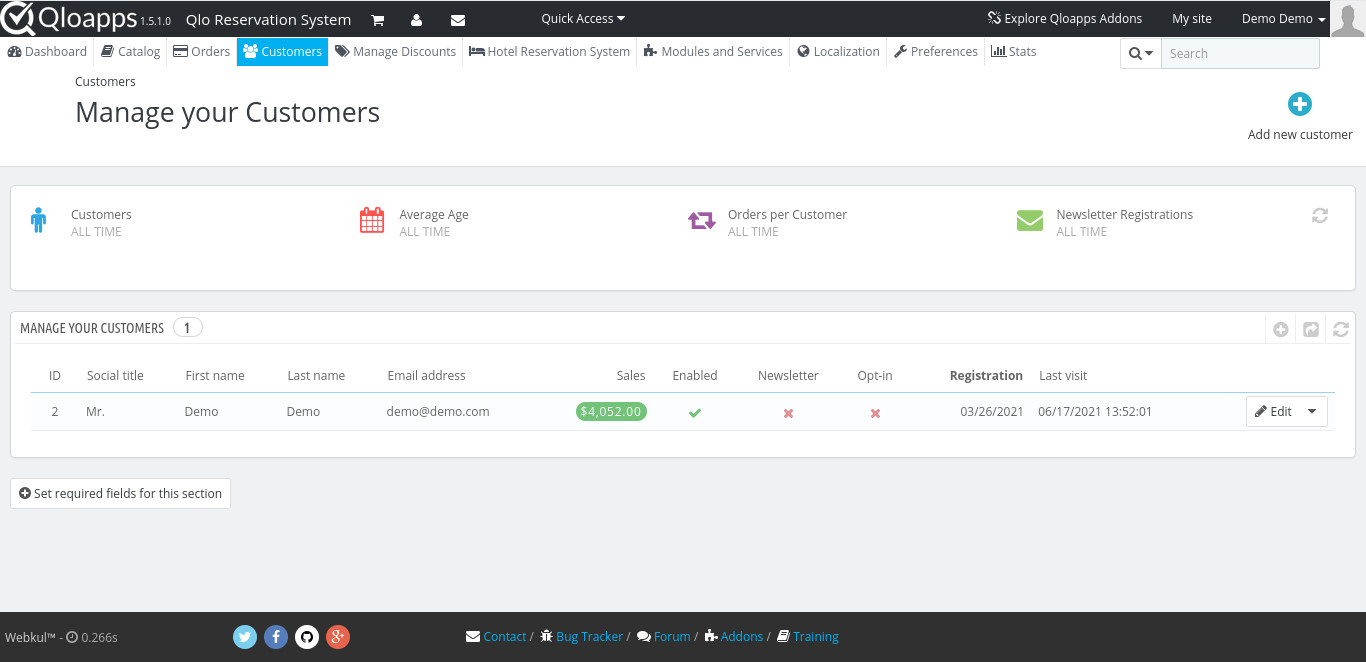
\includegraphics[scale=.5]{imagenes/estado_arte/qlo.png}}
    \caption{Interfaz gráfica de Qlo Hotel \& Booking Reservation}
    \label{fig}
\end{figure}

Esta alternativa podría funcionar aunque con ciertos límites. Entre sus limitaciones algunas como el no poder guardar información personalizada de las personas o que tengan que ser los ``clientes'' los que se asocien a una habitación podría limitar el trabajo de la fundación.

De aplicaciones para gestionar actividades hay más alternativas libres. La mayoría de alternativas ofrecen los que busca la asociación: gestión de actividades, cuentas para residentes, etc. Una de las características que no incluye ninguna de las alternativas libres analizadas es la puntuación y ranking de asistentes, uno de los aspectos diferenciales que la fundación busca perseguir. Algunas de las más interesantes son Agorakit, Gancio o Mobilizon.

En cuanto a alternativas no libres o de pago, es difícil encontrar alternativas asequibles o con planes de precios especializados para organizaciones sin ánimo de lucro. Esto se puede ver como algo normal debido a que está orientado principalmente a un sector comercial.

Finalmente, analizando varias alternativas y diferentes tipos de producto, creo que no existe uno que consiga satisfacer las necesidades de la fundación. Hay varios ``puntos flacos'' que ningun software de los analizados cumple, los cuales formarán parte de las características diferenciales de la alternativa a realizar:

\begin{itemize}
    \item Adaptación total de los datos recogidos a cada una de las personas asociadas con la fundación.
    \item Conexión entre las gestión de las personas de la fundación y su participación en las actividades propuestas por esta.
    \item Gestión de citas de personas, algo que no estaba contemplado en la mayoría de productos debido al estar representadas las personas más como clientes que como residentes.
    \item Búsqueda avanzada en base a las características de los usuarios.
    \item Acceso a estadísticas de la fundación en base a parámetros especificados por ellos mismos.
\end{itemize}

A partir de esto, habiendo analizando y escuchado las preferencias de la organización, lo mejor será el desarrollo de una aplicación móvil personalizada para la propia fundación, incluyendo las características deseadas por esta y adaptándola a su flujo de trabajo.
	
	\chapter{Planificación}

\section{Metodología utilizada}


\section{Temporización}

\section{Seguimiento del desarrollo}


	% Análisis del problema
	% 1. Análisis de requisitos
	% 2. Análisis de las soluciones
	% 3. Solucion propuesta
	% 4. Análisis de seguridad
	\chapter{Análisis del problema}

%%%%%%%%%%%%%%%%%%%%%%%%%%%%%%%%%%%%%%%
% REQUISITOS DEL PROYECTO
%%%%%%%%%%%%%%%%%%%%%%%%%%%%%%%%%%%%%%%

\section{Requisitos}

Tras las diferentes reuniones con los clientes, se desarrollaron una serie de exigencias y requisitos que tendrá que cumplir la aplicación y el sistema. Para un mejor entendimiento y desglose, estos se han separado por tipo de requisitos y dentro de esto por las diferentes secciones de la aplicación. Estas secciones serán: la gestión de personas que contendrá todo lo referente a las personas almacenadas en el sistema y las acciones a realizar sobre estas, gestión de alojamientos que contendrá lo relacionado con las casas gestionadas por la fundación, así como los residentes de cada una de estas y la gestión de actividades, con lo referente a las actividades y talleres organizados por la organización.  

\subsection{Requisitos funcionales}

\begin{enumerate}[start=1,label={RF-\arabic*.}]

    \item La aplicación contemplará tres secciones: gestión de personas, gestión de alojamiento y gestión de actividades.
    \item Cada usuario que use el sistema tendrá que identificarse con unas credenciales únicas.
    \item Existirán 4 roles de usuario que restringirán que actividades podrán o no hacer. Estos serán: administrador, estándar, invitado y participante.
    \item Los usuarios con el rol de administrador serán los únicos que podrán crear, modificar y eliminar a otros usuarios, así como modificar sus roles.
    \item Los usuarios con el rol de invitado podrán tener restringido el acceso a cualquiera de las secciones.
    \item Los usuarios con el rol de participante solo tendrán acceso a la sección de actividades.
    \item El sistema contemplará una opción de exportación de los datos de personas y de ocupación, a diferentes formatos (csv y excel).
    \item Las estadísticas (\ref{rf-es-personas}, \ref{rf-es-ocupacion}) podrán mostrarse de forma total o filtradas por periodos de tiempo (semanas, meses, años...).

\end{enumerate}

\subsubsection{Gestión de personas}

\begin{enumerate}[start=9,label={RF-\arabic*.}]

    \item Existirán cuatro tipos de personas en el sistema: residentes, voluntarios, socios y colaboradores.
    \item Se podrán añadir y eliminar personas del sistema.
    \item Se podrá modificar cualquier dato de las personas del sistema.
    \item Se podrán añadir y eliminar documentos asociados a una persona.
    \item Se podrán dar de alta y de baja a los residentes más de una vez. Se considera un alta cuando entran a residir en la fundación y una baja cuando la abandonan.
    \item La información de cada uno de los residentes se seguirá almacenando en el sistema aunque se le haya dado de baja de la fundación, con la excepción de que un administrador decida eliminar a esa persona del sistema. 
    \item Los usuarios con el rol de administrador podrán:
    \begin{itemize}
        \item Añadir y eliminar personas del sistema.
        \item Dar de alta y de baja a personas.
        \item Modificar los datos de una persona.
        \item Añadir y eliminar documentos asociados a una persona.
        \item Consultar los datos de cualquier persona del sistema.
        \item Crear y eliminar usuarios del sistema.
    \end{itemize}
    \item Los usuarios con el rol estándar podrán:
        \begin{itemize}
            \item Dar de alta y de baja a personas.
            \item Añadir personas al sistema.
            \item Consultar datos de las personas.
            \item Consultar los documentos de las personas.
        \end{itemize}
    \item Los usuarios con el rol invitado podrán:
        \begin{itemize}
            \item Consultar los datos de las personas
            \item Consultar los documentos de las personas
        \end{itemize}
    \item Los usuarios con el rol de participante no podrán acceder a esta sección.
    \item El acceso a la información por parte de los usuarios con el rol de invitados podrá estar limitada en cuanto a tipos de personas.
    \item El sistema contemplará búsquedas de personas por cualquiera de los datos asociados a estas o colectivos a los que pertenezcan.
    \item Se contemplarán búsquedas mixtas e individuales, es decir, búsquedas dentro de un tipo de persona concreto, o búsquedas de cualquier tipo de persona sobre campos coincidentes (búsqueda por nombre, ocupación etc.).
    \item Los documentos asociados a las personas serán de tipo imagen o documento de texto (pdf, doc, odt).
    \item A la hora de añadir una fotografía desde la aplicación, se proporcionará una cámara nativa además de incluir la opción de agregarla desde la galería de imágenes del smartphone.
    \item \label{rf-es-personas} La aplicación tendrá un apartado dedicado a mostrar estadísticas sobre:
        \begin{itemize}
            \item Número de residentes totales de la fundación.
            \item Número de residentes filtrados por género.
            \item Número de residentes menores.
            \item Número de residentes hijos de otro residente.
            \item Número de madres y padres.
            \item Número de residentes filtrados por colectivo al que pertenecen.
            \item Número de voluntarios.
            \item Número de socios.
            \item Número de colaboradores.
            \item Número de personas empadronadas.
            \item Número de personas con documentación arreglada.
        \end{itemize}
    \item Se contemplará un sistema de citas asociadas a cada residente de la fundación:
        \begin{itemize}
            \item Se almacenarán citas importantes asociadas a cada uno de los residentes.
            \item Se notificará a través de la aplicación a los usuarios con los roles de administrador y estándar un día antes de la cita y el mismo día de esta.
            \item Se notificará a por email al residente un día antes de la cita y el mismo día de esta.
            \item Los usuarios con los roles de administrador y estándar podrán ver las próximas citas.
        \end{itemize}
    \item Los datos de las personas se exportarán en tres archivos diferentes, uno por cada tipo de persona (residentes, voluntarios, colaboradores y socios)
    \item Para cada persona se exportarán todos los datos almacenados de estos.

\end{enumerate}

\subsubsection{Gestión de alojamiento}

\begin{enumerate}[start=26,label={RF-\arabic*.}]

    \item Se podrán añadir, eliminar y modificar casas en el sistema.
    \item Se podrán añadir, eliminar y modificar habitaciones dentro de las casas.
    \item Se podrán añadir, eliminar y modificar residentes de las habitaciones.
    \item Se podrá cambiar de casa o habitación a los residentes.
    \item Existirá una ocupación para cada habitación.
    \item Los usuarios con el rol de administrador en tema de alojamientos podrán:
        \begin{enumerate}
            \item Añadir y eliminar casas.
            \item Añadir o eliminar habitaciones dentro de las casas.
            \item Modificar la casa o habitación de un residente.
            \item Consultar los residentes que ocupan una casa o habitación.
        \end{enumerate}
    \item Los usuarios con el rol estándar en tema de alojamientos podrán:
        \begin{enumerate}
            \item Asignar una casa o habitación a un residente que no tengan ninguna asignada ya.
            \item Consultar los residentes que ocupan una casa o habitación. 
        \end{enumerate}
    \item Los usuarios con el rol de invitados solo podrán ver quien ocupa cada casa/habitación.
    \item Los usuarios con el rol de participante no podrán acceder a la sección de alojamientos.
    \item \label{rf-es-ocupacion} Las estadísticas que debe cubrir la aplicación sobre los alojamientos serán:
        \begin{itemize}
            \item Porcentaje de ocupación actual de las casas.
            \item Número de plazas libres sobre el total.
            \item Número de casas con alguna plaza libre.
        \end{itemize}    
    \item Los datos a exportar serán todos los asociados a cada casa, junto con las personas que las ocupan.

\end{enumerate}

\subsubsection{Gestión de actividades}

\begin{enumerate}[start=37,label={RF-\arabic*.}]

    \item Los usuarios con el rol de administrador podrán:
        \begin{itemize}
            \item Añadir nuevas actividades.
            \item Eliminar actividades.
            \item Ver actividades disponibles.
            \item Ver la información de cualquier actividad.
            \item Puntuar a los asistentes de una actividad.
        \end{itemize}
    \item Los usuarios con el rol estándar podrán:
        \begin{itemize}
            \item Añadir nuevas actividades.
            \item Ver actividades disponibles.
            \item Ver la información de cualquier actividad.
            \item Puntuar a los asistentes de una actividad.
        \end{itemize}
    \item Los usuarios con el rol de asistente podrán:
        \begin{itemize}
            \item Apuntarse a actividades.
            \item Desapuntarse de actividades.
            \item Ver actividades disponibles.
            \item Ver la información de cualquier actividad.
            \item Ver las estadísticas de su participación en actividades, así como el ranking con respecto a otros participantes.
        \end{itemize}
    \item Las estadísticas que cubrirá la aplicación para cada individuo será:
        \begin{itemize}
            \item Actividades realizadas
            \item Puntuación media de las actividades
            \item Puntuación individual en cada una de las actividades realizada.
        \end{itemize}
    \item Existirá un ranking de usuarios en base a la puntuación total de todas las actividades realizadas por cada uno de los usuarios.
    \item Existirán diferentes divisiones en base a la puntuación de cada usuario:
        \begin{itemize}
            \item Bronce: Menos de 10 puntos.
            \item Plata: Entre 10 y 50 puntos.
            \item Oro: Entre 50 y 150 puntos.
            \item Platino: Más de 150 puntos.
        \end{itemize}

\end{enumerate}

\subsection{Requisitos no funcionales}

\begin{enumerate}[start=1,label={RNF-\arabic*.}]
    \item \label{rnf-plataformas}La aplicación debe estar desarrollada tanto para Android como para IOS.
    \item Todos los usuarios, menos los del rol de invitado, estarán asociados a un residente.
    \item Todos los datos se transmitirán y almacenarán de forma segura, evitando así exponer información delicada.
    \item Los datos de carácter sensible no se almacenarán nunca en el dispositivo del usuario.
    \item Todo el sistema tendrá que cumplir con la Ley Orgánica 3/2018, de 5 de diciembre, de Protección de Datos Personales y garantía de los derechos digitales.
\end{enumerate}

\subsubsection{Gestión de personas}

\begin{enumerate}[start=6,label={RNF-\arabic*.}]

    \item Cada persona tendrá asociados datos personales, así como documentos.
    \item Los datos asociados de los residentes serán:
        \begin{itemize}
            \item Nombre y apellidos
            \item Documento identificativo (DNI, pasaporte...)
            \item Fecha de nacimiento
            \item Genero
            \item Email
            \item Teléfono móvil con prefijo
            \item Nacionalidades
            \item País de nacimiento
            \item País de procedencia
            \item Fotografía
            \item Fechas de ingreso
            \item Fechas de baja
            \item Motivo de baja
            \item Estado civil
            \item Colaborador allegado (Colaborador que ha traído a esta persona a la fundación)
            \item Formación (ESO, Bachillerato...)
            \item Ocupación
            \item Factores de riesgo
            \item Si tiene o no el permiso de trabajo
            \item Un valor identificativo del estado de su documentación española
            \item Un valor identificativo del estado de su empadronamiento en caso de que esté residiendo en ese momento
            \item Un valor identificativo del estado de su tarjeta sanitaria
            \item Residente de la fundación del que es hijo o hija
            \item Residente de la fundación del que es padre o madre
            \item Colectivos a los que pertenecen
        \end{itemize}
    \item Los datos asociados de los voluntarios serán:
        \begin{itemize}
            \item Nombre y apellidos
            \item Documento identificativo (DNI, pasaporte...)
            \item Fecha de nacimiento
            \item Género
            \item Email
            \item Nacionalidad
            \item Fotografía
            \item Dirección
            \item Ciudad
            \item País
            \item Nacionalidad
            \item Teléfono
            \item Conocimientos
            \item Preferencias
            \item Idiomas
            \item Disponibilidad de mañanas
            \item Disponibilidad de tardes
            \item Disponibilidad de fines de semana
            \item Fechas de llegada
            \item Fechas de salida
            \item Experiencias previas
        \end{itemize} 
        
    \item Los conocimientos de un voluntario/colaborador posibles serán: informática, diseño web, cocina, agricultura, guardería, albañilería, fontanería u otros en caso de que el usuario que los quiera especificar.
    \item Las preferencias de un voluntario serán seleccionadas sobre los conocimientos previamente indicados.
    \item Los datos asociados de los colaboradores serán:
        \begin{itemize}
            \item Nombre y apellidos
            \item Documento identificativo (DNI, pasaporte...)
            \item Fecha de nacimiento
            \item Género
            \item Email
            \item Nacionalidad
            \item Dirección
            \item Ciudad
            \item País
            \item Edad
            \item Teléfono
        \end{itemize}
    \item Los datos asociados a los socios serán:
        \begin{itemize}
            \item Nombre y apellidos
            \item Fecha de inicio
            \item Cuota
            \item Relación con otro socio
            \item Email
            \item Indicador si quiere recibir una newsletter
        \end{itemize}
    \item El sistema seguirá almacenando los datos de las personas a pesar de su baja en la fundación.
    \item Todos los teléfonos almacenados en el sistema tendrán el prefijo del país correspondiente.
    \item Los datos asociados a una cita serán los siguientes:
        \begin{itemize}
            \item Título de la cita
            \item Descripción de la cita
            \item Fecha y hora de la cita
        \end{itemize}

\end{enumerate}

\subsubsection{Gestión de alojamiento}

\begin{enumerate}[start=15,label={RNF-\arabic*.}]

    \item Cada casa estará identificada por un número.
    \item Cada casa tendrá un nombre asociado.
    \item Cada habitación estará identificada por un número único en base a las demás habitaciones dentro de la misma casa, además de un número único en referencia a las demás habitaciones.
    \item Cada habitación tendrá un número de plazas y una ocupación (residentes actuales).

\end{enumerate}

\subsubsection{Gestión de actividades}

\begin{enumerate}[start=18,label={RNF-\arabic*.}]

    \item Cada actividad tendrá asociada la siguiente información:
        \begin{itemize}
            \item Nombre
            \item Foto de la actividad
            \item Descripción
            \item Fecha
            \item Asistentes de una actividad
            \item Puntuación de los asistentes a la actividad
        \end{itemize}
    \item La puntuación de un residente en una actividad será de un mínimo de 0 y un máximo de 10.

\end{enumerate}
 

	% Desarrollo bajo sprints: 
	% 	1. Permitir registros y login de usuarios
	% 	2. Desarrollo del sistema de incidencias
	% 	3. Desarrollo del sistema de denuncias administrativas y accidentes
	% 	4. Desarrollo del sistema de croquis
	%   5. Instalación de la aplicación de manera automática
	\chapter{Implementación}

\section{Sistema de autenticación}

La protección del sistema y de los datos es algo fundamental en este proyecto. Cada usuario debe tener acceso a distintos recursos en base a su rol y se debe garantizar que un agente no registrado no pueda acceder al sistema. Para esto, se ha utilizado un sistema de autenticación basado en tokens. Esta era una alternativa que no dependía de otros servicios de autenticación externos y era lo suficientemente extendida para proporcionar una correcta seguridad al sistema. Junto con esto, esta alternativa es una de las más estandarizadas en la protección de APIs.

El funcionamiento es básico. Al usuario se le proporciona un token, firmado por una clave secreta en el proceso de login (representado en la Figura \ref{fig:ds-login}). A esta clave solo tendrá acceso el proceso correspondiente del servidor. Este token tendrá información cifrada acerca de la sesión, lo que permitirá que al realizar la autorización de acceso, no se tenga que validar la información del usuario accediendo a la base de datos, cosa que ralentizaría bastante el tiempo de respuesta del servidor. El usuario con este token podrá realizar peticiones, dentro de sus permisos. El funcionamiento de la autorización se explica esquemáticamente en el diagrama de secuencia de la Figura \ref{fig:ds-auth}.

\begin{figure}[]
    \centering
    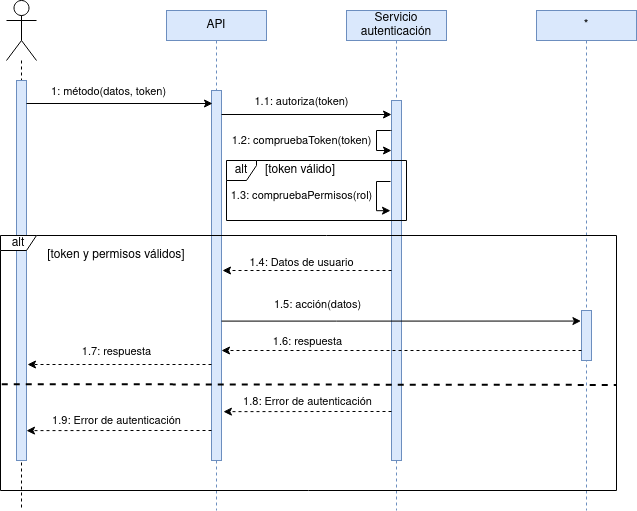
\includegraphics[width=\textwidth]{diseno/sistema/DS/autorizacion.png}
    \caption{Autorización del sistema}
    \label{fig:ds-auth}
\end{figure}

\begin{figure}[]
    \centering
    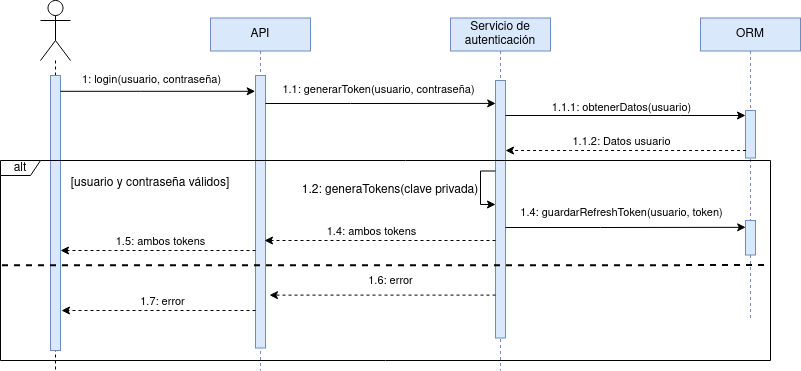
\includegraphics[width=\textwidth]{diseno/sistema/DS/login.png}
    \caption{Inicio de sesión en el sistema}
    \label{fig:ds-login}
\end{figure}

El token de autorización tiene una ``caducidad'' de 15 minutos. Esto será necesario debido a que, si el token no tuviese caducidad, un usuario eliminado o con los permisos modificados, podría seguir accediendo a zonas no autorizadas. Este tiempo ha sido elegido en base al tiempo de uso estimado por sesión. 

Para evitar que el usuario tenga que introducir su usuario y contraseña cada 15 minutos, se utiliza otro tipo de token. Este token será igual que el de autorización pero con la principal diferencia de que no caducará. Su utilidad será la de generar un nuevo token de autorización. Al generar un nuevo token de autorización, se comprobará la información del usuario en la base de datos, para proporcionar información de sesión actualizada en el nuevo token de autorización. El funcionamiento del token de refresh está esquemáticamente explicado en el diagrama de secuencia de la Figura \ref{fig:ds-refresh}.

\begin{figure}[]
    \centering
    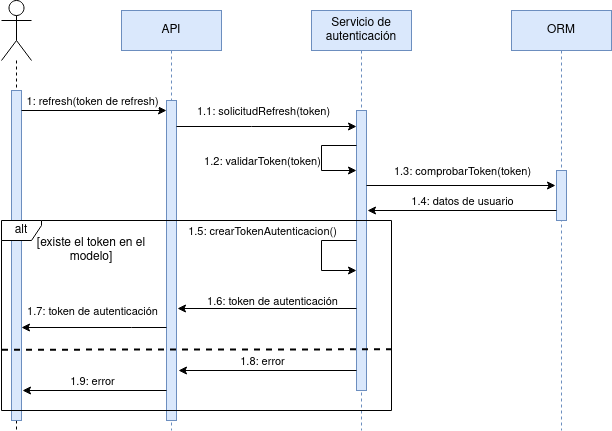
\includegraphics[width=\textwidth]{diseno/sistema/DS/refresh.png}
    \caption{Funcionamiento del token de refresh}
    \label{fig:ds-refresh}
\end{figure}

Los tokens de refresh válidos hasta el momento se almacenarán en la base de datos. Esto será así para que el usuario pueda invalidar los tokens mediante un cierre de sesión. El proceso de ``logout'' es el mostrado en la Figura \ref{fig:ds-logout}.   

\begin{figure}[]
    \centering
    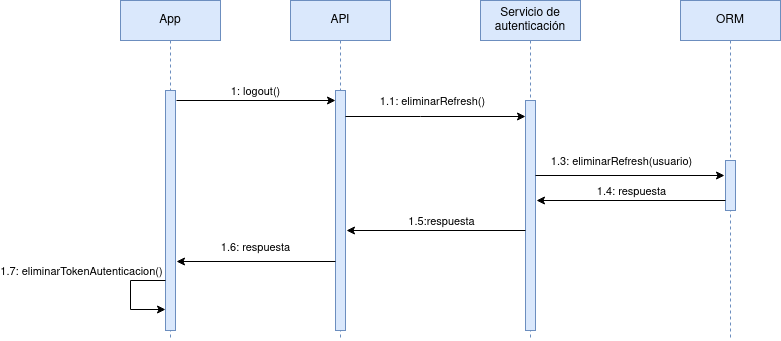
\includegraphics[width=\textwidth]{diseno/sistema/DS/logout.png}
    \caption{Cierre de sesión en el sistema}
    \label{fig:ds-logout}
\end{figure}

Todo esto permitirá controlar los usuarios actualmente logueados en el sistema, así como borrar usuarios, prohibiendo su acceso al eliminar su información del sistema, así como su token de refresh. Al editar un usuario, también garantizamos que como mucho, en los próximos 15 minutos estos cambios sean efectivos.

Todo el mecanismo de autorización se ha implementado con el objetivo de controlar correctamente los permisos de acceso de los usuarios, sin ver el rendimiento y el tiempo de respuesta del servidor afectado. 

	% Presupuesto

	% Conclusiones
	\chapter{Conclusiones y trabajos futuros}



	% Trabajos futuros


	
	\newpage
	\bibliography{bibliografia}
	\bibliographystyle{plain}
	
\end{document}

